\chapter{Blocchi costruttivi digitali}
Nei capitoli precedenti è stata esaminata la progettazione delle reti combinatorie e sequenziali usando le espressioni booleane. In questo capitolo vengono introdotti blocchi costruttivi sia combinatori sia sequenziali più complessi, utilizzati nei sistemi digitali.

\section{Circuiti aritmetici}
I circuiti aritmetici sono i blocchi costruttivi centrali dei calcolatori. I calcolatori e la logica digitale eseguono molte funzioni aritmetiche come addizioni, sottrazioni, confronti, traslazioni, moltiplicazioni e divisioni. In questo paragrafo viene descritta la realizzazione hardware per ognuna di queste operazioni.

\subsection{Addizione}
L’addizione è una delle operazioni più comuni nei sistemi digitali. Inizieremo ad esaminare come sia possibile sommare due numeri binari a 1 bit. Per poi estendere l’operazione ai numeri binari ad N bit.

\subsubsection*{Half Adder}
Si comincia dalla costruzione di un semisommatore (half adder) a 1 bit. 
\begin{figure}[ht]
    \centering
    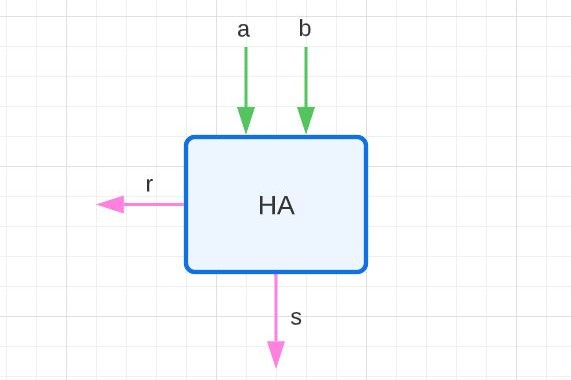
\includegraphics[width = 8cm]{images/half_adder.JPG}
    \caption{Semisommatore o Half Adder}
    \label{fig:half_adder}
\end{figure}
Come mostrato in Figura \ref{fig:half_adder}, il semisommatore ha due ingressi, A e B, e due uscite, S e R. S rappresenta la somma di A e B. Se A e B hanno valore 1, S è uguale a 2, un valore che non può essere rappresentato con una sola cifra binaria. Di conseguenza, il valore 2 viene rappresentato con un riporto (carry) R nella colonna successiva. Il semisommatore può essere costruito con una porta XOR e una porta AND.
\begin{table}[H]
    \centering
    \begin{tabular}{c|c}
         abc & rs \\\hline
         000 & 00\\
         001 & 01\\
         010 & 01\\
         011 & 10
    \end{tabular}
    \caption{Tavola di verità dell'Half Adder}
    \label{tab:half_adder}
\end{table}

\subsubsection*{Full Adder}
Un sommatore completo (full adder), è formato dalla concatenazione di più half adder e accetta in ingresso il valore c come mostrato nella Figura \ref{fig:full_adder}.
\begin{figure}[H]
    \centering
    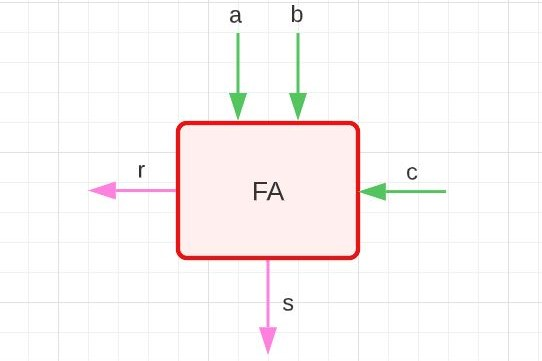
\includegraphics[width = 8cm]{images/full_adder.JPG}
    \caption{Sommatore completo o Full Adder}
    \label{fig:full_adder}
\end{figure}

\begin{table}[H]
    \centering
    \begin{tabular}{c|c}
         abc & rs \\\hline
         000 & 00\\
         001 & 01\\
         010 & 01\\
         011 & 10\\\hline
         100 & 01\\
         101 & 10\\
         110 & 10\\
         111 & 11
    \end{tabular}
    \caption{Tavola di verità del Full Adder}
    \label{tab:full_adder}
\end{table}

\subsubsection*{Ripple Carry Adder}
Un sommatore a N bit somma due ingressi a N bit: A e B. A questi aggiunge c, S per ottenere un risultato ad N bit e un riporto R. Questo sommatore viene comunemente chiamato sommatore a propagazione di riporto (o RCA, ripple carry adder) perché il riporto di un bit si propaga nel bit successivo.

Il metodo più semplice per costruire un sommatore a propagazione di riporto è collegare in cascata N full adder completi. In questo modo, R di uno stadio fa riferimento a c dello stadio successivo, come mostrato in Figura \ref{fig:ripple_carry_adder}.

\begin{figure}[H]
    \centering
    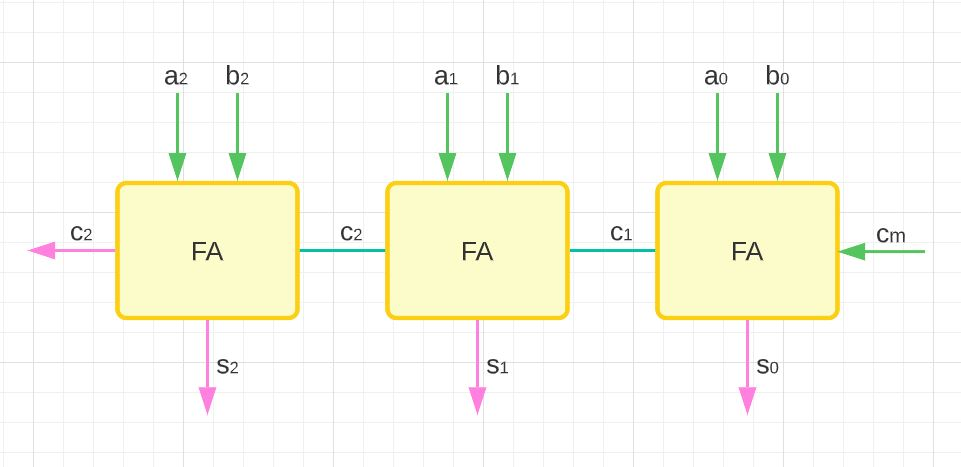
\includegraphics[width = 12cm]{images/ripple_carry_adder.JPG}
    \caption{Sommatore a propagazione di riporto o Ripple Carry Adder}
    \label{fig:ripple_carry_adder}
\end{figure}

Notiamo che se l'ultima somma genera un riporto c, allora si produce overflow. 

\subsection{Sottrazione}
I sommatori sono in grado di sommare numeri sia positivi sia negativi utilizzando la rappresentazione dei numeri in complemento a due. La sottrazione è quindi facile quanto l’addizione: si inverte il segno del secondo numero e poi si esegue la somma. Il cambio di segno di un numero in complemento a due si esegue negando tutti i bit e aggiungendo un 1.

Ad esempio se si vuole calcolare $Y = A - B$, per prima cosa si crea il numero in complemento a due di $B$: si negano tutti i bit di $B$ per ottenere $\overline{B}$ e si aggiunge 1 per ottenere $-B = B + 1$. Questo valore viene aggiunto ad $A$ per ottenere $Y=A-B+1=A-B$. Questo risultato può essere ottenuto con l’utilizzo di un sommatore a propagazione di riporto facendo la somma $A + B$ con $c = 1$.

\begin{description}
    \item[N.B.] Per usare RCA con la sottrazione abbiamo bisogno di un segnale distinto che ci permette di specificare l'operazione da compiere ($0$: addizione, $1$: sottrazione).
\end{description}

\subsection{Comparatori}
Un comparatore determina se due numeri binari sono uguali o se uno dei due è maggiore o minore dell’altro. Un comparatore riceve due numeri binari a N bit, A e B. La comparazione di valore dei numeri con segno viene solitamente effettuata calcolando A – B e guardando il segno (cioè il bit più significativo) del risultato dell’operazione. Se il risultato è negativo (cioè se il bit del segno è uguale a 1) allora A è minore di B. Al contrario, se il risultato è positivo, A è maggiore o uguale a B.

\section{Moduli notevoli}
Vediamo ora come sono strutturati i principali moduli di un elaboratore. Questi moduli possono essere combinati tra di loro per svolgere in maniera più veloce le funzioni desiderate.

\subsection{Decodificatore}
Un decodificatore è un modulo formato da $n$ ingressi e $2^n$ uscite, di cui solo una di queste vale 1.

\begin{center}
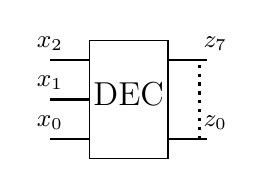
\begin{tikzpicture}
    \draw [fill=white] (0,0) rectangle (1,1.5);
    \draw [-,thick] (0,0.25) -- (-0.5,0.25);
    \draw [-,thick] (0,0.75) -- (-0.5,0.75);
    \draw [-,thick] (0,1.25) -- (-0.5,1.25);
    \draw [-,thick] (1,0.25) -- (1.5,0.25);
    \draw [-,thick] (1,1.25) -- (1.5,1.25);
    \draw[very thick, dotted] (1.4,0.25) -- (1.4,1.25);
    % lecter
    \draw (-0.5,0.25) -- (-0.5,0.25) node [above] {\small{$x_0$}};
    \draw (-0.5,0.75) -- (-0.5,0.75) node [above] {\small{$x_1$}};
    \draw (-0.5,1.25) -- (-0.5,1.25) node [above] {\small{$x_2$}};
    \draw (1.6,0.25) -- (1.6,0.25) node [above] {\small{$z_0$}};
    \draw (1.6,1.25) -- (1.6,1.25) node [above] {\small{$z_7$}};
    \draw (0.5,0.55) -- (0.5,0.55) node [above] {\large{DEC}};
\end{tikzpicture}
\end{center}

\begin{table}[ht]
    \centering
    \begin{tabular}{ccc|cccccccc}
        $x_2$&$x_1$&$x_0$ & $z_0$&$z_1$&$z_2$&$z_3$&$z_4$&$z_5$&$z_6$&$z_7$\\\hline
        0&0&0 & 1&0&0&0&0&0&0&0 \\
        0&0&1 & 0&1&0&0&0&0&0&0 \\
        0&1&0 & 0&0&1&0&0&0&0&0 \\
        0&1&1 & 0&0&0&1&0&0&0&0 \\\hline
        1&0&0 & 0&0&0&0&1&0&0&0 \\
        1&0&1 & 0&0&0&0&0&1&0&0 \\
        1&1&0 & 0&0&0&0&0&0&1&0 \\
        1&1&1 & 0&0&0&0&0&0&0&1 \\
    \end{tabular}
    \caption{Tavola del decodificatore}
    \label{tab:decodific}
\end{table}
Notiamo come la tavola del decodificatore \ref{tab:decodific} è facilmente realizzabile attraverso la diagonale di 1.
Quindi le equazioni delle uscite saranno:
\begin{itemize}
    \item[] $z_0=\overline{x_2}\overline{x_1}\overline{x_0}$
    \item[] $z_1=\overline{x_2}\overline{x_1}x_0$
    \item[] ...
    \item[] $z_7=x_2x_1x_0$
\end{itemize}

\begin{center}
    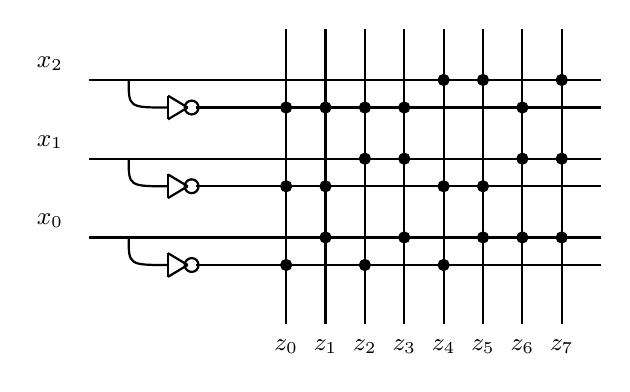
\begin{tikzpicture}
        % x line
        \draw [thick] (1.35,0) -- (6.5,0);
        \draw [thick] (0,0.35) -- (6.5,0.35);
        \draw [thick] (1.35,1) -- (6.5,1);
        \draw [thick] (0,1.35) -- (6.5,1.35);
        \draw [thick] (1.35,2) -- (6.5,2);
        \draw [thick] (0,2.35) -- (6.5,2.35);
        % y line
        \draw [thick] (2.5,-0.75) -- (2.5,3);
        \draw [thick] (3,-0.75) -- (3,3);
        \draw [thick] (3.5,-0.75) -- (3.5,3);
        \draw [thick] (4,-0.75) -- (4,3);
        \draw [thick] (4.5,-0.75) -- (4.5,3);
        \draw [thick] (5,-0.75) -- (5,3);
        \draw [thick] (5.5,-0.75) -- (5.5,3);
        \draw [thick] (6,-0.75) -- (6,3);
        % curve line
        \draw[thick] (0.5,1.35) .. controls (0.5,1) .. (1,1);
        \draw[thick] (0.5,0.35) .. controls (0.5,0) .. (1,0);
        \draw[thick] (0.5,2.35) .. controls (0.5,2) .. (1,2);
        % triangle and point
        \draw [thick] (1,-0.15) -- (1,0.15);\draw [thick] (1,-0.15) -- (1.25,0);\draw [thick] (1,0.15) -- (1.25,0);
        \draw [thick] (1,0.85) -- (1,1.15);\draw [thick] (1,0.85) -- (1.25,1);\draw [thick] (1,1.15) -- (1.25,1);
        \draw [thick] (1,1.85) -- (1,2.15);\draw [thick] (1,1.85) -- (1.25,2);\draw [thick] (1,2.15) -- (1.25,2);
        \draw[thick, black] (1.30,0) circle (2.5pt);\draw[thick, black] (1.30,1) circle (2.5pt);\draw[thick, black] (1.30,2) circle (2.5pt);
        % lecter
        \draw (-0.5,2.35) -- (-0.5,2.35) node [above] {\small{$x_2$}};
        \draw (-0.5,1.35) -- (-0.5,1.35) node [above] {\small{$x_1$}};
        \draw (-0.5,0.35) -- (-0.5,0.35) node [above] {\small{$x_0$}};
        \draw (2.5,-1.25) -- (2.5,-1.25) node [above] {\small{$z_0$}};\draw (3,-1.25) -- (3,-1.25) node [above] {\small{$z_1$}};
        \draw (3.5,-1.25) -- (3.5,-1.25) node [above] {\small{$z_2$}};\draw (4,-1.25) -- (4,-1.25) node [above] {\small{$z_3$}};
        \draw (4.5,-1.25) -- (4.5,-1.25) node [above] {\small{$z_4$}};\draw (5,-1.25) -- (5,-1.25) node [above] {\small{$z_5$}};
        \draw (5.5,-1.25) -- (5.5,-1.25) node [above] {\small{$z_6$}};\draw (6,-1.25) -- (6,-1.25) node [above] {\small{$z_7$}};
        % black point
        \filldraw[black] (2.5,0) circle (2pt);\filldraw[black] (2.5,1) circle (2pt);\filldraw[black] (2.5,2) circle (2pt);
        \filldraw[black] (3,0.35) circle (2pt);\filldraw[black] (3,1) circle (2pt);\filldraw[black] (3,2) circle (2pt);
        \filldraw[black] (3.5,0) circle (2pt);\filldraw[black] (3.5,1.35) circle (2pt);\filldraw[black] (3.5,2) circle (2pt);
        \filldraw[black] (4,0.35) circle (2pt);\filldraw[black] (4,1.35) circle (2pt);\filldraw[black] (4,2) circle (2pt);
        \filldraw[black] (4.5,0) circle (2pt);\filldraw[black] (4.5,1) circle (2pt);\filldraw[black] (4.5,2.35) circle (2pt);
        \filldraw[black] (5,0.35) circle (2pt);\filldraw[black] (5,1) circle (2pt);\filldraw[black] (5,2.35) circle (2pt);
        \filldraw[black] (5.5,0.35) circle (2pt);\filldraw[black] (5.5,1.35) circle (2pt);\filldraw[black] (5.5,2) circle (2pt);
        \filldraw[black] (6,0.35) circle (2pt);\filldraw[black] (6,1.35) circle (2pt);\filldraw[black] (6,2.35) circle (2pt);
    \end{tikzpicture}
\end{center}

\subsection{Codificatore}
Il codificatore è un modulo formato da $n$ ingressi, di cui solo uno vale 1, e $\log_2n$ uscite.
Il codificatore fornisce in uscita la codifica binaria dell'unica linea di ingresso 1.

\begin{center}
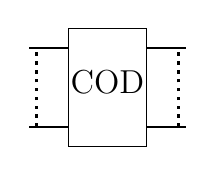
\begin{tikzpicture}
    \draw [fill=white] (0,0) rectangle (1,1.5);
    \draw [-,thick] (1,0.25) -- (1.5,0.25);
    \draw [-,thick] (1,1.25) -- (1.5,1.25);
    \draw [-,thick] (0,0.25) -- (-0.5,0.25);
    \draw [-,thick] (0,1.25) -- (-0.5,1.25);
    \draw[very thick, dotted] (1.4,0.25) -- (1.4,1.25);
    \draw[very thick, dotted] (-0.4,0.25) -- (-0.4,1.25);
    % lecter
    \draw (0.5,0.55) -- (0.5,0.55) node [above] {\large{COD}};
\end{tikzpicture}
\end{center}

\begin{table}[ht]
    \centering
    \begin{tabular}{cccc|cc}
         $x_3$&$x_2$&$x_1$&$x_0$ & $z_1$&$z_0$\\\hline
         0&0&0&1 & 0&0\\
         0&0&1&0 & 0&1\\
         0&1&0&0 & 1&0\\
         1&0&0&0 & 1&1\\
    \end{tabular}
    \caption{Tavola del codificatore}
    \label{tab:codific}
\end{table}

Le equazioni di output saranno:
\begin{itemize}
    \item[] $z_0=x_1+x_3$
    \item[] $z_1=x_2+x_3$
\end{itemize}

\begin{center}
    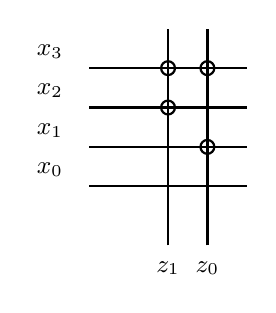
\begin{tikzpicture}
        % x line
        \draw [thick] (0,0) -- (2,0);
        \draw [thick] (0,0.5) -- (2,0.5);
        \draw [thick] (0,1) -- (2,1);
        \draw [thick] (0,1.5) -- (2,1.5);
        % y line
        \draw [thick] (1,-0.75) -- (1,2);
        \draw [thick] (1.5,-0.75) -- (1.5,2);
        % lecter
        \draw (-0.5,1.5) -- (-0.5,1.5) node [above] {\small{$x_3$}};\draw (-0.5,1) -- (-0.5,1) node [above] {\small{$x_2$}};
        \draw (-0.5,0.5) -- (-0.5,0.5) node [above] {\small{$x_1$}};\draw (-0.5,0) -- (-0.5,0) node [above] {\small{$x_0$}};
        \draw (1,-1.25) -- (1,-1.25) node [above] {\small{$z_1$}};\draw (1.5,-1.25) -- (1.5,-1.25) node [above] {\small{$z_0$}};
        % point
        \draw[thick, black] (1.5,0.5) circle (2.5pt);\draw[thick, black] (1,1) circle (2.5pt);
        \draw[thick, black] (1,1.5) circle (2.5pt);\draw[thick, black] (1.5,1.5) circle (2.5pt);
    \end{tikzpicture}
\end{center}

\subsection{Transcodificatore}
Un transcodificatore è formato da un decodificatore e da un codificatore inseriti a cascata.
Il transcodificatore avrà quindi $n$ ingressi ed $n$ uscite.

\begin{center}
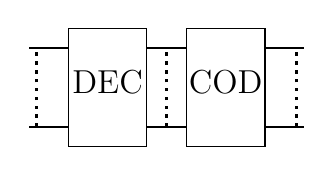
\begin{tikzpicture}
    \draw [fill=white] (0,0) rectangle (1,1.5);
    \draw [-,thick] (1,0.25) -- (1.5,0.25);
    \draw [-,thick] (1,1.25) -- (1.5,1.25);
    \draw [-,thick] (0,0.25) -- (-0.5,0.25);
    \draw [-,thick] (0,1.25) -- (-0.5,1.25);
    \draw[very thick, dotted] (1.25,0.25) -- (1.25,1.25);
    \draw[very thick, dotted] (-0.4,0.25) -- (-0.4,1.25);
    \draw [fill=white] (1.5,0) rectangle (2.5,1.5);
    \draw [-,thick] (2.5,0.25) -- (3,0.25);
    \draw [-,thick] (2.5,1.25) -- (3,1.25);
    \draw[very thick, dotted] (2.9,0.25) -- (2.9,1.25);
    % lecter
    \draw (0.5,0.55) -- (0.5,0.55) node [above] {\large{DEC}};
    \draw (2,0.55) -- (2,0.55) node [above] {\large{COD}};
\end{tikzpicture}
\end{center}

\subsubsection*{Transcodificatore a sette segmenti}
Con il transcodificatore a sette segmenti (chiamato così per il numero di segmenti che formano ogni numero da 0 a 9) è un particolare tipo di transcodificatore che permette di rappresentare un numero binario con la codifica tramite rappresentazione decimale.

\begin{center}
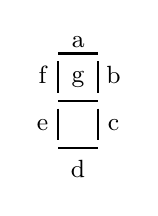
\begin{tikzpicture}
    \draw [thick] (0,0) -- (0.5,0);
    \draw [thick] (0,0.6) -- (0.5,0.6);\draw [thick] (0,-0.6) -- (0.5,-0.6);
    \draw [thick] (0,0.1) -- (0,0.5);\draw [thick] (0,-0.1) -- (0,-0.5);
    \draw [thick] (0.5,0.1) -- (0.5,0.5);\draw [thick] (0.5,-0.1) -- (0.5,-0.5);
    % lecter
    \draw (0.25,0.55) -- (0.25,0.55) node [above] {\small{a}};\draw (0.25,-1.1) -- (0.25,-1.1) node [above] {\small{d}};
    \draw (-0.2,0.1) -- (-0.2,0.1) node [above] {\small{f}};\draw (0.7,0.1) -- (0.7,0.1) node [above] {\small{b}};
    \draw (-0.2,-0.5) -- (-0.2,-0.5) node [above] {\small{e}};\draw (0.7,-0.5) -- (0.7,-0.5) node [above] {\small{c}};
    \draw (0.25,0.05) -- (0.25,0.05) node [above] {\small{g}};
\end{tikzpicture}
\end{center}

Tramite questo schema possiamo rappresentare tutti i numeri da 0 a 9. Ad esempio il numero 4 sarà formato da $b,c,f,g$ e verrà pertanto rappresentato nel seguente modo:
\begin{table}[ht]
    \centering
    \begin{tabular}{|cccc|ccccccc|}
         \hline$x_3$&$x_2$&$x_1$&$x_0$& $a$&$b$&$c$&$d$&$e$&$f$&$g$\\\hline\hline
         0&1&0&0 & 0&1&1&0&0&1&1\\\hline
    \end{tabular}
\end{table}

\subsection{Multiplexer}
Il multiplexer è formato da $n$ linee di ingressi di dati, $\log_2n$ ingressi a selezione (o controllo), di cui solo uno di questi vale 1, e una sola uscita.
La funzione fornisce in uscita la linea di dati associata all'unica linea di controllo uguale a 1.

\begin{center}
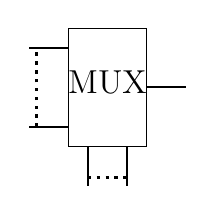
\begin{tikzpicture}
    \draw [fill=white] (0,0) rectangle (1,1.5);
    \draw [-,thick] (0,0.25) -- (-0.5,0.25);
    \draw [-,thick] (0,1.25) -- (-0.5,1.25);
    \draw[very thick, dotted] (-0.4,0.25) -- (-0.4,1.25);
    \draw [-,thick] (1,0.75) -- (1.5,0.75);
    \draw [-,thick] (0.25,0) -- (0.25,-0.5);
    \draw [-,thick] (0.75,0) -- (0.75,-0.5);
    \draw[very thick, dotted] (0.25,-0.4) -- (0.75,-0.4);
    % lecter
    \draw (0.5,0.55) -- (0.5,0.55) node [above] {\large{MUX}};
\end{tikzpicture}
\end{center}

Un MUX é costituito da una porta OR, che riceve le uscite di n porte AND, le quali funzionano da interruttori; infine, un decodificatore attiva l’interruttore selezionato dai segnali di controllo.

\subsubsection*{Multiplexer per funzioni booleane}
Notiamo come il multiplexer può essere utilizzato per rappresentare le funzioni booleane. Il tutto sarà più chiaro con un esempio.
\begin{example}
    \begin{table}[ht]
        \centering
        \begin{tabular}{c|c}
             $abc$ & $f$\\\hline
             000 & 0\\
             001 & 1\\
             010 & 0\\
             011 & 1\\\hline
             100 & 1\\
             101 & 1\\
             110 & 1\\
             111 & 0
        \end{tabular}
    \end{table}
    Per rappresentarlo fisso i valori della funzione sugli ingressi e uso le variabili come segnali di controllo.
    Ottenendo così in ingresso una sequenza di 0 e 1: $01011110$, in cotrollo le tre variabili $a,b,c$ e in uscita la funzione $f$.
    
    Lo stesso concetto è applicabile rappresentandolo come funzione di 3 variabili ma con un MUX di 4. A differenza di prima avremo quindi come controllo le variabili $a,b$, come ingresso i 4 valori che identificano nella tabella la funzione quando ad esempio a e b valgono 0, a vale 0 e b vale 1 ... e come uscita la funzione $f$.

    \begin{center}
    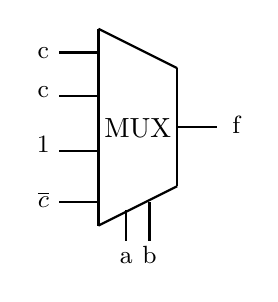
\begin{tikzpicture}
        % trapezio
        \draw [-,thick] (0,0) -- (0,2.5);
        \draw [-,thick] (1,0.5) -- (1,2);
        \draw [-,thick] (0,0) -- (1,0.5);
        \draw [-,thick] (0,2.5) -- (1,2);
        % ingressi, condizioni e uscite
        \draw [-,thick] (0,2.2) -- (-0.5,2.2);\draw [-,thick] (0,0.3) -- (-0.5,0.3);
        \draw [-,thick] (0,1.65) -- (-0.5,1.65);\draw [-,thick] (0,0.95) -- (-0.5,0.95);
        \draw [-,thick] (0.35,0.2) -- (0.35,-0.2);\draw [-,thick] (0.65,0.3) -- (0.65,-0.2);
        \draw [-,thick] (1,1.25) -- (1.5,1.25);
        % lecter
        \draw (0.5,1) -- (0.5,1) node [above] {\normalsize{MUX}};\draw (1.75,1.05) -- (1.75,1.05) node [above] {\small{f}};
        \draw (0.35,-0.6) -- (0.35,-0.6) node [above] {\small{a}};\draw (0.65,-0.6) -- (0.65,-0.6) node [above] {\small{b}};
        \draw (-0.7,2) -- (-0.7,2) node [above] {\small{c}};\draw (-0.7,0.1) -- (-0.7,0.1) node [above] {\small{$\overline{c}$}};
        \draw (-0.7,1.5) -- (-0.7,1.5) node [above] {\small{c}};\draw (-0.7,0.8) -- (-0.7,0.8) node [above] {\small{1}};
    \end{tikzpicture}
    \end{center}
\end{example}

Infatti per $a$ e $b$ presi a due a due nella tabella nei primi quattro casi vale $c$, nei successivi due vale $1$ e negli ultimi due vale $\overline{c}$.

\subsection{Demultiplexer}
Il demultiplexer è formato da una linea di ingresso, $\log_2n$ linee di controllo, di cui solo una vale 1, e $n$ linee in uscita.
La funzione fornisce l'unico ingresso sulla linea di uscita selezionata dall'unica linea di controllo 1.
\begin{center}
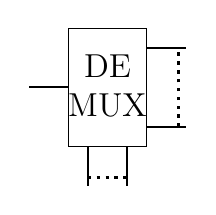
\begin{tikzpicture}
    \draw [fill=white] (0,0) rectangle (1,1.5);
    \draw [-,thick] (1,0.25) -- (1.5,0.25);
    \draw [-,thick] (1,1.25) -- (1.5,1.25);
    \draw[very thick, dotted] (1.4,0.25) -- (1.4,1.25);
    \draw [-,thick] (0,0.75) -- (-0.5,0.75);
    \draw [-,thick] (0.25,0) -- (0.25,-0.5);
    \draw [-,thick] (0.75,0) -- (0.75,-0.5);
    \draw[very thick, dotted] (0.25,-0.4) -- (0.75,-0.4);
    % lecter
    \draw (0.5,0.75) -- (0.5,0.75) node [above] {\large{DE}};
    \draw (0.5,0.25) -- (0.5,0.25) node [above] {\large{MUX}};
\end{tikzpicture}
\end{center}

Un DEMUX é costituito da n porte AND, le quali funzionano da interruttori, e da un decodificatore che attiva l’interruttore selezionato dai segnali di controllo.

Anche in questo caso si possono inserire multiplexer e demultiplexer in cascata.

\subsection{ROM}

Una ROM (Read Only Memory) è un dispositivo con $n$ ingressi (dette linee di indirizzamento) ed $m$ uscite (dette linee dati). 
All'interno del dispositivo, le linee di indirizzamento selezionano una fra $2^n$ righe di una matrice $2^n×m$.
La selezione della riga i-esima della matrice consente di leggere, su ciascuna delle $m$ linee dati, il valore binario memorizzato nella cella.
E’ la composizione di un decodificatore e un codificatore generalizzato cioè di una matrice di AND (le cui entrate sono le linee di indirizzamento e le cui uscite sono le entrate di una matrice di OR) e di una matrice di OR (le cui uscite sono le linee dati).

Il nome ROM (read-only memory) deriva dal fatto che questo modulo combinatorio può essere visto come una memoria (cioè un insieme di celle di dimensione fissata, ognuna con un suo proprio indirizzo) e non riscrivibile (quindi, di sola lettura).

\begin{example}\label{es:rom}
    Data la seguente traccia: rappresenta $x$ in Ca2 da 3 bit con $x\in[-4;2]$ realizzare la ROM avente output: $$y=\begin{cases}2x\text{ se }x>0\\x+2\text{ altrimenti}\end{cases}$$.
    
    Ricaviamo la tavola di verità dalla traccia:
    \begin{table}[ht]
        \centering
        \begin{tabular}{cc|c}
             &$x_0x_1x_2$&$y_3y_2y_1y_0$\\\hline
             0 & 000 & 0010\\
             1 & 001 & 0010\\
             2 & 010 & 0100\\
             - & 011 & ----\\\hline
             -4 & 100 & 1110\\
             -3 & 101 & 1111\\
             -2 & 110 & 0000\\
             -1 & 111 & 0001\\
        \end{tabular}
        \caption{Tavola di verità della ROM}
        \label{tab:es:rom}
    \end{table}
    
    La ROM sarà così rappresentata:
    
    \begin{center}
    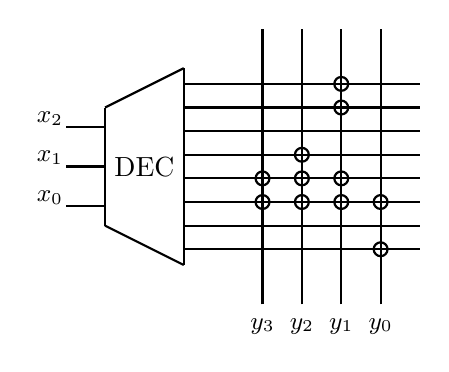
\begin{tikzpicture}
        % trapezio
        \draw [-,thick] (0,0.5) -- (0,2);
        \draw [-,thick] (1,0) -- (1,2.5);
        \draw [-,thick] (0,0.5) -- (1,0);
        \draw [-,thick] (0,2) -- (1,2.5);
        % ingressi, condizioni e uscite
        \draw [-,thick] (0,1.75) -- (-0.5,1.75);\draw [-,thick] (0,0.75) -- (-0.5,0.75);\draw [-,thick] (0,1.25) -- (-0.5,1.25);
        % lecter
        \draw (0.5,1) -- (0.5,1) node [above] {\normalsize{DEC}};
        
        \draw (-0.7,0.65) -- (-0.7,0.65) node [above] {\small{$x_0$}};\draw (-0.7,1.15) -- (-0.7,1.15) node [above] {\small{$x_1$}};\draw (-0.7,1.65) -- (-0.7,1.65) node [above] {\small{$x_2$}};
        
        \draw (2,-1) -- (2,-1.) node [above] {\small{$y_3$}};\draw (2.5,-1) -- (2.5,-1.) node [above] {\small{$y_2$}};\draw (3,-1) -- (3,-1.) node [above] {\small{$y_1$}};\draw (3.5,-1) -- (3.5,-1.) node [above] {\small{$y_0$}};
        % line
        \draw [-,thick] (1,0.2) -- (4,0.2);\draw [-,thick] (1,0.5) -- (4,0.5);
        \draw [-,thick] (1,0.8) -- (4,0.8);\draw [-,thick] (1,1.1) -- (4,1.1);
        \draw [-,thick] (1,1.4) -- (4,1.4);\draw [-,thick] (1,1.7) -- (4,1.7);
        \draw [-,thick] (1,2) -- (4,2);\draw [-,thick] (1,2.3) -- (4,2.3);
        
        \draw [-,thick] (2,-0.5) -- (2,3);\draw [-,thick] (2.5,-0.5) -- (2.5,3);
        \draw [-,thick] (3,-0.5) -- (3,3);\draw [-,thick] (3.5,-0.5) -- (3.5,3);
        
        % point
        \draw[thick, black] (2,0.8) circle (2.5pt);\draw[thick, black] (2,1.1) circle (2.5pt);
        \draw[thick, black] (2.5,0.8) circle (2.5pt);\draw[thick, black] (2.5,1.1) circle (2.5pt);\draw[thick, black] (2.5,1.4) circle (2.5pt);
        \draw[thick, black] (3,0.8) circle (2.5pt);\draw[thick, black] (3,1.1) circle (2.5pt);\draw[thick, black] (3,2) circle (2.5pt);\draw[thick, black] (3,2.3) circle (2.5pt);
        \draw[thick, black] (3.5,0.2) circle (2.5pt);\draw[thick, black] (3.5,0.8) circle (2.5pt);
    \end{tikzpicture}
    \end{center}
    
\end{example}

\subsection{PLA}
Il PLA o Programmable Logic Array serve per ottenere insiemi di funzioni booleane. E' formato da una matrice di AND, che produce i termini prodotto di funzioni in forma minimale, seguita da una matrice di OR con tante linee quante sono le funzioni da produrre. In tal senso una PLA è più efficiente di una ROM.

\begin{example}
    Ripredendo l'Esempio \ref{es:rom}, calcoliamo le espressioni minimali con le K-mappe:
    \begin{table}[ht]
        \centering
        \begin{tabular}{|c|c|c|c|c|}
            \hline \diagbox[width=1.5cm]{$x_0$}{$x_1x_2$} & 00 & 01 & 11 & 10 \\\hline\hline
            0 & 0 & 0 & 0 & 0\\\hline
            1 & 1 & 1 & 0 & 0\\\hline
        \end{tabular}
        \caption{$y_3 = x_2\overline{x_1}$}
    \end{table}
    \begin{table}[ht]
        \centering
        \begin{tabular}{|c|c|c|c|c|}
            \hline \diagbox[width=1.5cm]{$x_0$}{$x_1x_2$} & 00 & 01 & 11 & 10 \\\hline\hline
            0 & 0 & 0 & - & 1\\\hline
            1 & 1 & 1 & 0 & 0\\\hline
        \end{tabular}
        \caption{$y_2 = x_2\overline{x_1}+\overline{x_2}x_1$}
    \end{table}
    \begin{table}[ht]
        \centering
        \begin{tabular}{|c|c|c|c|c|}
            \hline \diagbox[width=1.5cm]{$x_0$}{$x_1x_2$} & 00 & 01 & 11 & 10 \\\hline\hline
            0 & 1 & 1 & - & 0\\\hline
            1 & 1 & 1 & 0 & 0\\\hline
        \end{tabular}
        \caption{$y_1 = \overline{x_1}$}
    \end{table}
    \begin{table}[H]
        \centering
        \begin{tabular}{|c|c|c|c|c|}
            \hline \diagbox[width=1.5cm]{$x_0$}{$x_1x_2$} & 00 & 01 & 11 & 10 \\\hline\hline
            0 & 0 & 0 & - & 0\\\hline
            1 & 0 & 1 & 1 & 0\\\hline
        \end{tabular}
        \caption{$y_0 = x_2x_0$}
    \end{table}
    
    Rappresentiamo ora il PLA:
    \begin{center}
    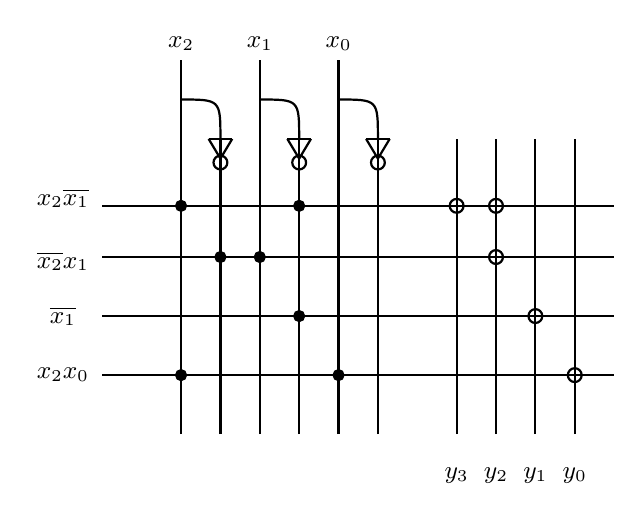
\begin{tikzpicture}
        
        % x line
        \draw [thick] (1.5,0) -- (8,0);
        \draw [thick] (1.5,0.75) -- (8,0.75);
        \draw [thick] (1.5,1.5) -- (8,1.5);
        \draw [thick] (1.5,2.15) -- (8,2.15);
        
        % y line
        \draw [thick] (2.5,-0.75) -- (2.5,4);
        \draw [thick] (3,-0.75) -- (3,3);
        \draw [thick] (3.5,-0.75) -- (3.5,4);
        \draw [thick] (4,-0.75) -- (4,3);
        \draw [thick] (4.5,-0.75) -- (4.5,4);
        \draw [thick] (5,-0.75) -- (5,3);
        
        \draw [thick] (6,-0.75) -- (6,3);
        \draw [thick] (6.5,-0.75) -- (6.5,3);
        \draw [thick] (7,-0.75) -- (7,3);
        \draw [thick] (7.5,-0.75) -- (7.5,3);
        
        % curve line
        \draw[thick] (3,3) .. controls (3,3.5) .. (2.5,3.5);
        \draw[thick] (4,3) .. controls (4,3.5) .. (3.5,3.5);
        \draw[thick] (5,3) .. controls (5,3.5) .. (4.5,3.5);
        
        % triangle and point
        \draw [thick] (2.85,3) -- (3.15,3);\draw [thick] (2.85,3) -- (3,2.75);\draw [thick] (3.15,3) -- (3,2.75);
        \draw [thick] (3.85,3) -- (4.15,3);\draw [thick] (3.85,3) -- (4,2.75);\draw [thick] (4.15,3) -- (4,2.75);
        \draw [thick] (4.85,3) -- (5.15,3);\draw [thick] (4.85,3) -- (5,2.75);\draw [thick] (5.15,3) -- (5,2.75);
        \draw[thick, black] (3,2.7) circle (2.5pt);\draw[thick, black] (4,2.7) circle (2.5pt);\draw[thick, black] (5,2.7) circle (2.5pt);
        
        % lecter
        \draw (1,2) -- (1,2) node [above] {\small{$x_2\overline{x_1}$}};
        \draw (1,1.2) -- (1,1.2) node [above] {\small{$\overline{x_2}x_1$}};
        \draw (1,0.5) -- (1,0.5) node [above] {\small{$\overline{x_1}$}};
        \draw (1,-0.2) -- (1,-0.2) node [above] {\small{$x_2x_0$}};
        
        \draw (2.5,4) -- (2.5,4) node [above] {\small{$x_2$}};\draw (3.5,4) -- (3.5,4) node [above] {\small{$x_1$}};\draw (4.5,4) -- (4.5,4) node [above] {\small{$x_0$}};
        
        \draw (6,-1.5) -- (6,-1.5) node [above] {\small{$y_3$}};\draw (6.5,-1.5) -- (6.5,-1.5) node [above] {\small{$y_2$}};\draw (7.5,-1.5) -- (7.5,-1.5) node [above] {\small{$y_0$}};\draw (7,-1.5) -- (7,-1.5) node [above] {\small{$y_1$}};
        
        % black point
        \filldraw[black] (2.5,0) circle (2pt);\filldraw[black] (2.5,2.15) circle (2pt);
        \filldraw[black] (3,1.5) circle (2pt);\filldraw[black] (3.5,1.5) circle (2pt);
        \filldraw[black] (4,0.75) circle (2pt);\filldraw[black] (4,2.15) circle (2pt);
        \filldraw[black] (4.5,0) circle (2pt);
        
        \draw[thick, black] (6,2.15) circle (2.5pt);\draw[thick, black] (6.5,2.15) circle (2.5pt);\draw[thick, black] (6.5,1.5) circle (2.5pt);
        \draw[thick, black] (7,0.75) circle (2.5pt);\draw[thick, black] (7.5,0) circle (2.5pt);
    \end{tikzpicture}
\end{center}
\end{example}

Per apprfondire vedi Esercizio \ref{es:rom_pla}

\newpage
\section{Esercizi svolti}

\begin{exercise}\label{es:rom_pla}
    Dato il seguente multiplexer trova:\begin{enumerate}
        \item Le esperessioni di $f_1$ e $f_2$;
        \item La tavola di verità;
        \item La ROM;
        \item Il PLA.
    \end{enumerate}
    \begin{center}
    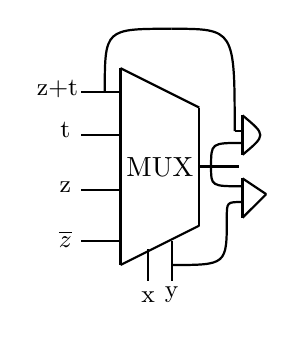
\begin{tikzpicture}
        % trapezio
        \draw [-,thick] (0,0) -- (0,2.5);
        \draw [-,thick] (1,0.5) -- (1,2);
        \draw [-,thick] (0,0) -- (1,0.5);
        \draw [-,thick] (0,2.5) -- (1,2);
        % ingressi, condizioni e uscite
        \draw [-,thick] (0,2.2) -- (-0.5,2.2);\draw [-,thick] (0,0.3) -- (-0.5,0.3);
        \draw [-,thick] (0,1.65) -- (-0.5,1.65);\draw [-,thick] (0,0.95) -- (-0.5,0.95);
        \draw [-,thick] (0.35,0.2) -- (0.35,-0.2);\draw [-,thick] (0.65,0.3) -- (0.65,-0.2);
        \draw [-,thick] (1,1.25) -- (1.5,1.25);
        % curve line
        \draw[thick] (-0.2,2.2) .. controls (-0.2,3) .. (0.65,3);\draw[thick] (0.65,3) .. controls (1.45,3) .. (1.45,1.7);
        \draw[thick] (1.45,1.7) .. controls (1.45,1.7) .. (1.55,1.7);
        \draw[thick] (1.15,1.25) .. controls (1.15,1.55) .. (1.55,1.55);
        
        \draw[thick] (0.65,0) .. controls (1.35,0) .. (1.35,0.6);\draw[thick] (1.35,0.6) .. controls (1.35,0.8) .. (1.55,0.8);
        \draw[thick] (1.15,1.25) .. controls (1.15,1) .. (1.55,1);
        % altro
        \draw [-,thick] (1.55,1.4) -- (1.55,1.9);\draw[thick] (1.55,1.4) .. controls (1.85,1.65) .. (1.55,1.9);
        \draw [-,thick] (1.55,0.6) -- (1.55,1.1);\draw [-,thick] (1.55,0.6) -- (1.85,0.9);\draw [-,thick] (1.55,1.1) -- (1.85,0.9);
        % lecter
        \draw (0.5,1) -- (0.5,1) node [above] {\normalsize{MUX}};
        \draw (0.35,-0.6) -- (0.35,-0.6) node [above] {\small{x}};\draw (0.65,-0.6) -- (0.65,-0.6) node [above] {\small{y}};
        \draw (-0.8,2) -- (-0.8,2) node [above] {\small{z+t}};\draw (-0.7,0.1) -- (-0.7,0.1) node [above] {\small{$\overline{z}$}};
        \draw (-0.7,1.5) -- (-0.7,1.5) node [above] {\small{t}};\draw (-0.7,0.8) -- (-0.7,0.8) node [above] {\small{z}};
    \end{tikzpicture}
    \end{center}
    
    \begin{enumerate}
        \item $f=(z+t)\overline{x}\overline{y}+t\overline{x}y+zx\overline{y}+\overline{z}xy$
        
        $f_1=f(z+t)=(z+t)\overline{x}\overline{y}+t\overline{x}y+zx\overline{y}+(t+\overline{z})xy$ Per idempotenza e assorbimento $= \overline{x}\overline{y}z+\overline{x}\overline{y}t+\overline{x}yt+x\overline{y}z+xyt+xy\overline{z}$ Elimino i termini non comuni
        \begin{center}
            $f_1=\overline{y}z+\overline{x}t+yt+xy\overline{z}$    
        \end{center}
        
        $f_2=f+y=\overline{x}\overline{y}z+\overline{x}\overline{y}t+\overline{x}yt+x\overline{y}z+xy\overline{z}+y$ Applico l'assorbimento $= \overline{x}\overline{y}z+\overline{x}\overline{y}t+x\overline{y}z+y$ Elimino i termini non comuni
        \begin{center}
            $f_2=\overline{y}z+\overline{x}\overline{y}t+y$
        \end{center}
    \end{enumerate}
    
    Rappresentiamo ora le nostre funzioni sulla tavola di verità:
    \begin{table}[H]
    \centering
    \begin{tabular}{c|c|c}
         xyzt & $f_1$&$f_2$\\\hline
         0000 & 0&0\\
         0001 & 1&1\\
         0010 & 1&1\\
         0011 & 1&1\\\hline
         0100 & 0&1\\
         0101 & 1&1\\
         0110 & 0&1\\
         0111 & 1&1\\\hline
         1000 & 0&0\\
         1001 & 0&0\\
         1010 & 1&1\\
         1011 & 1&1\\\hline
         1100 & 1&1\\
         1101 & 1&1\\
         1110 & 0&1\\
         1111 & 1&1\\
    \end{tabular}
    \caption{Tavola di verità}
\end{table}

    Con la ROM otteniamo un decodificatore con ingressi $x,y,z,y$ e 16 linee di uscita di $f_1$ e $f_2$ che formano la matrice di or.
    
    Troviamo le equazioni minimali con le K-mappe e successivamente il PLA:
    \begin{table}[H]
        \centering
        \begin{tabular}{|c|c|c|c|c|}
            \hline \diagbox[width=1.5cm]{$xy$}{$zt$} & 00 & 01 & 11 & 10 \\\hline\hline
            00 & 0 & 1 & 1 & 1\\\hline
            01 & 0 & 1 & 1 & 0\\\hline
            11 & 1 & 1 & 1 & 0\\\hline
            10 & 0 & 0 & 1 & 1\\\hline
        \end{tabular}
        \caption{$f_1 = yt+\overline{x}t+\overline{y}z+x\overline{y}z$}
    \end{table}
    \begin{table}[H]
        \centering
        \begin{tabular}{|c|c|c|c|c|}
            \hline \diagbox[width=1.5cm]{$xy$}{$zt$} & 00 & 01 & 11 & 10 \\\hline\hline
            00 & 0 & 1 & 1 & 1\\\hline
            01 & 1 & 1 & 1 & 1\\\hline
            11 & 1 & 1 & 1 & 1\\\hline
            10 & 0 & 0 & 1 & 1\\\hline
        \end{tabular}
        \caption{$f_2 = y+z+\overline{x}t$}
    \end{table}
    
    \begin{center}
    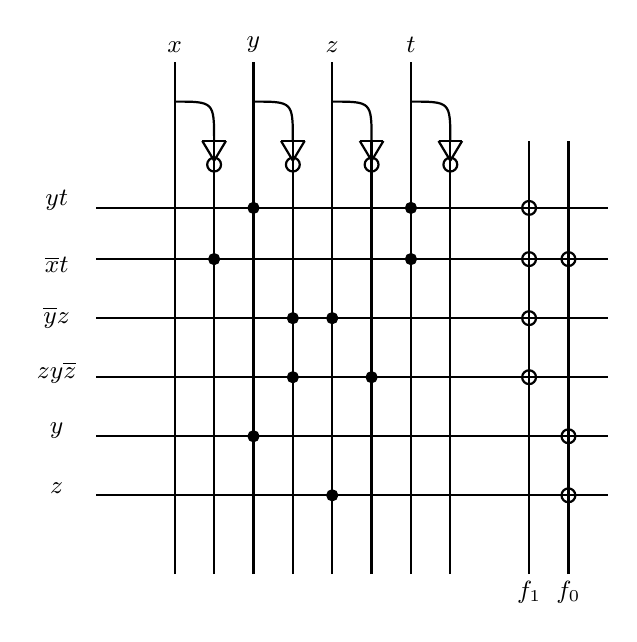
\begin{tikzpicture}
        
        % x line
        \draw [thick] (1.5,0) -- (8,0);
        \draw [thick] (1.5,0.75) -- (8,0.75);
        \draw [thick] (1.5,1.5) -- (8,1.5);
        \draw [thick] (1.5,2.15) -- (8,2.15);
        \draw [thick] (1.5,-0.75) -- (8,-0.75);
        \draw [thick] (1.5,-1.5) -- (8,-1.5);
        
        % y line
        \draw [thick] (2.5,-2.5) -- (2.5,4);
        \draw [thick] (3,-2.5) -- (3,3);
        \draw [thick] (3.5,-2.5) -- (3.5,4);
        \draw [thick] (4,-2.5) -- (4,3);
        \draw [thick] (4.5,-2.5) -- (4.5,4);
        \draw [thick] (5,-2.5) -- (5,3);
        \draw [thick] (5.5,-2.5) -- (5.5,4);
        \draw [thick] (6,-2.5) -- (6,3);
        
        \draw [thick] (7,-2.5) -- (7,3);
        \draw [thick] (7.5,-2.5) -- (7.5,3);
        
        % curve line
        \draw[thick] (3,3) .. controls (3,3.5) .. (2.5,3.5);
        \draw[thick] (4,3) .. controls (4,3.5) .. (3.5,3.5);
        \draw[thick] (5,3) .. controls (5,3.5) .. (4.5,3.5);
        \draw[thick] (6,3) .. controls (6,3.5) .. (5.5,3.5);
        
        % triangle and point
        \draw [thick] (2.85,3) -- (3.15,3);\draw [thick] (2.85,3) -- (3,2.75);\draw [thick] (3.15,3) -- (3,2.75);
        \draw [thick] (3.85,3) -- (4.15,3);\draw [thick] (3.85,3) -- (4,2.75);\draw [thick] (4.15,3) -- (4,2.75);
        \draw [thick] (4.85,3) -- (5.15,3);\draw [thick] (4.85,3) -- (5,2.75);\draw [thick] (5.15,3) -- (5,2.75);
        \draw [thick] (5.85,3) -- (6.15,3);\draw [thick] (5.85,3) -- (6,2.75);\draw [thick] (6.15,3) -- (6,2.75);
        \draw[thick, black] (3,2.7) circle (2.5pt);\draw[thick, black] (4,2.7) circle (2.5pt);\draw[thick, black] (5,2.7) circle (2.5pt);\draw[thick, black] (6,2.7) circle (2.5pt);
        
        % lecter
        \draw (1,2) -- (1,2) node [above] {\small{$yt$}};
        \draw (1,1.2) -- (1,1.2) node [above] {\small{$\overline{x}t$}};
        \draw (1,0.5) -- (1,0.5) node [above] {\small{$\overline{y}z$}};
        \draw (1,-0.2) -- (1,-0.2) node [above] {\small{$zy\overline{z}$}};
        \draw (1,-0.9) -- (1,-0.9) node [above] {\small{$y$}};
        \draw (1,-1.6) -- (1,-1.6) node [above] {\small{$z$}};
        
        \draw (2.5,4) -- (2.5,4) node [above] {\small{$x$}};\draw (3.5,4) -- (3.5,4) node [above] {\small{$y$}};\draw (4.5,4) -- (4.5,4) node [above] {\small{$z$}};\draw (5.5,4) -- (5.5,4) node [above] {\small{$t$}};
        
        \draw (7.5,-3) -- (7.5,-3) node [above] {\small{$f_0$}};\draw (7,-3) -- (7,-3) node [above] {\small{$f_1$}};
        
        % black point
        \filldraw[black] (3,1.5) circle (2pt);
        \filldraw[black] (3.5,2.15) circle (2pt);\filldraw[black] (3.5,-0.75) circle (2pt);
        \filldraw[black] (4,0.75) circle (2pt);\filldraw[black] (4,0) circle (2pt);
        \filldraw[black] (4.5,0.75) circle (2pt);\filldraw[black] (4.5,-1.5) circle (2pt);
        \filldraw[black] (5,0) circle (2pt);
        \filldraw[black] (5.5,1.5) circle (2pt);\filldraw[black] (5.5,2.15) circle (2pt);
        
        \draw[thick, black] (7,2.15) circle (2.5pt);\draw[thick, black] (7,1.5) circle (2.5pt);\draw[thick, black] (7,0.75) circle (2.5pt);\draw[thick, black] (7,0) circle (2.5pt);
        \draw[thick, black] (7.5,-1.5) circle (2.5pt);\draw[thick, black] (7.5,-0.75) circle (2.5pt);\draw[thick, black] (7.5,1.5) circle (2.5pt);
    \end{tikzpicture}
\end{center}
\end{exercise}